\renewenvironment{longtable}{\rowcolors{2}{LightGray}{white}\oldlongtable} {\endoldlongtable}
\chapter{GPIO操作及其中断}
\section{GPIO简介}
\ac{GPIO}是指通用目的输入输出设备。在STM32上,它以几组引脚的形式引出,可以连接其他电路组件,例如LED灯,此外,许多引脚有特定的复用功能,例如可以作为串口通信的Rx和Tx引脚,连接串口设备,例如GPS等。GPIO是STM32上最基本的外设,因此在这里我们首先来学习GPIO的一些基本应用,以此引出操作STM32外设的一般编程流程。
\par 
STM32的GPIO是一个比较高级的IO外设,不同于,每个引脚都支持几种不同的模式,适用于不同的应用场景,有的引脚还支持高达5V的输入电压。GPIO的基本电路结构如下图\footnote{截自\acs{RM}}。
\par 
\begin{figure}[h]
	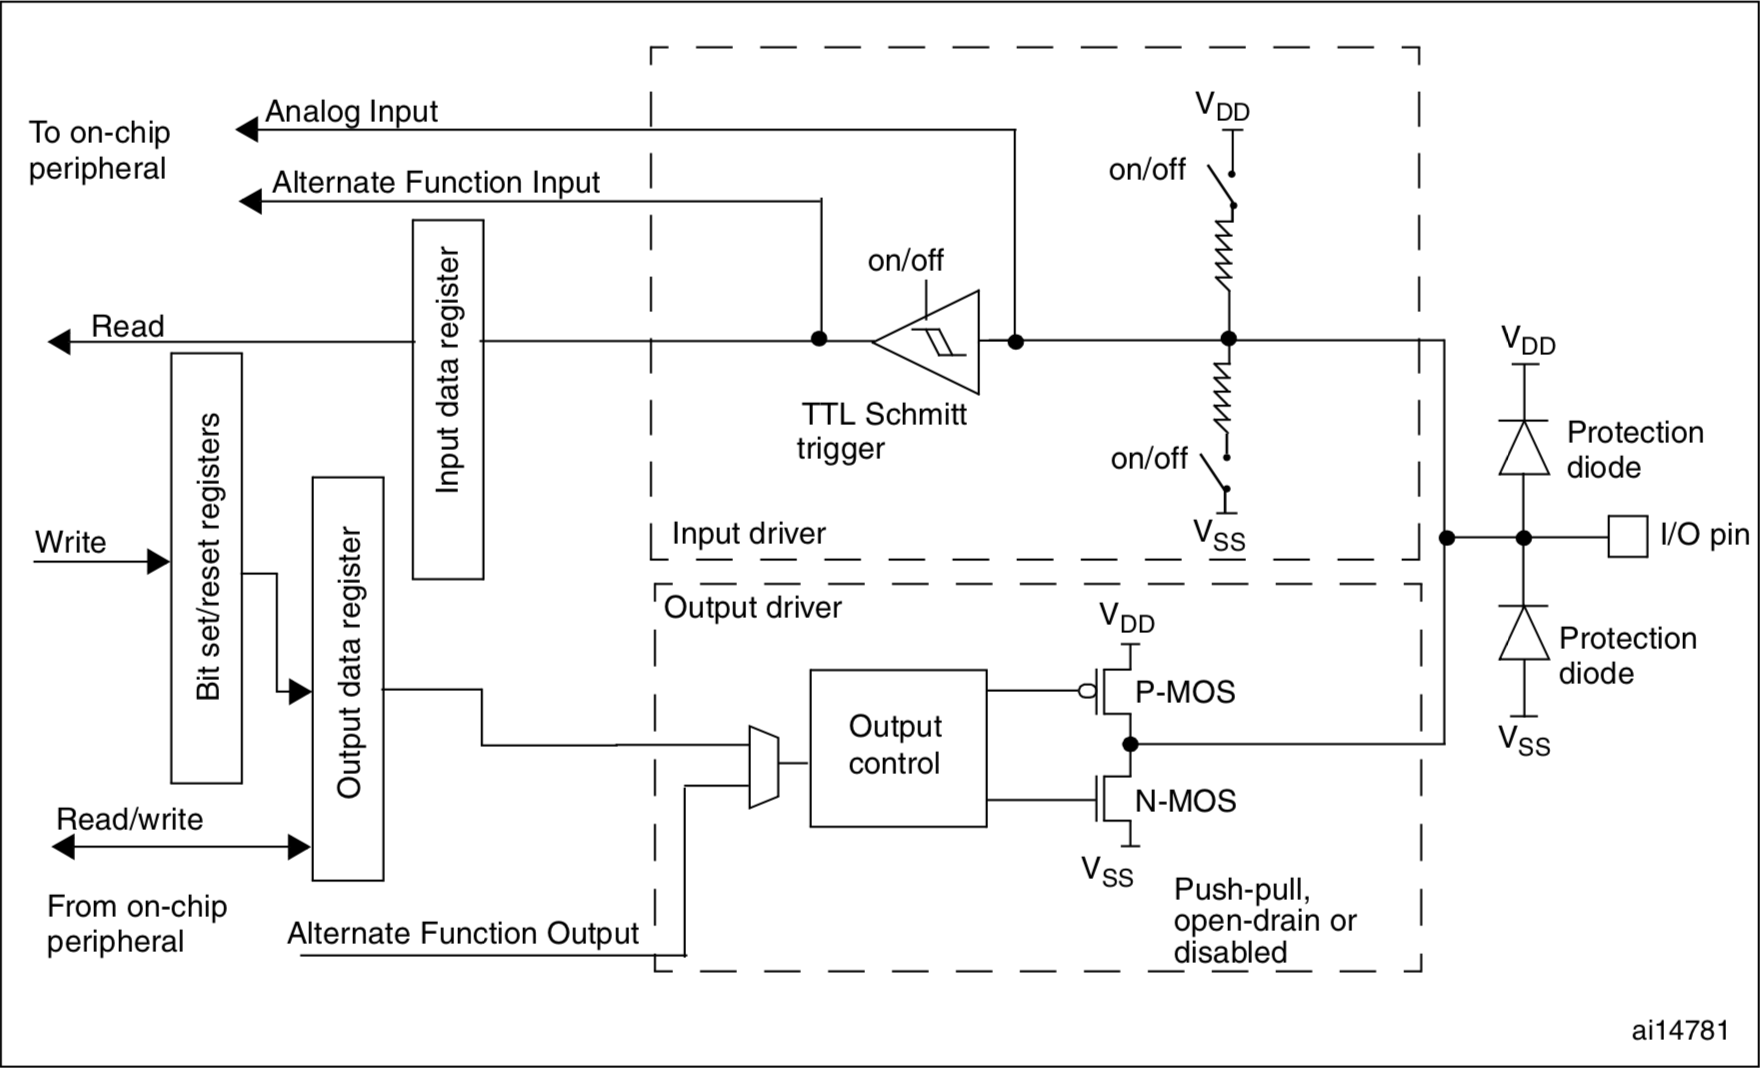
\includegraphics[width=\textwidth]{images/content/gpioCircuit.png}
	\captionof{figure}{GPIO基本结构}
	\label{fig:gpioCircuit}
\end{figure}
\par 
\newpage
GPIO支持的模式见下表:
\begin{center}
	\begin{longtable}[l]{| p{30mm} | p{40mm} | p{70mm} |}
		\caption{GPIO模式}\\
		\hline 
		\rowcolor{Gray}
		\textbf{类型} & \textbf{模式名称} & \textbf{简要描述} \\
		\hline
		\endfirsthead
		
		\hline 
		\rowcolor{Gray}
		\textbf{类型} & \textbf{模式名称} & \textbf{简要描述} \\
		\hline
		\endhead
		
		输出模式 & 推挽输出  & 电流较大的输出模式 \\
		输出模式 & 漏极开路输出 & 可以双向通信的输出模式,一般用于模拟通信协议(例如IIC) \\
		输出模式 & 复用推挽输出 & 作为复用功能时的推挽输出模式 \\
		输出模式 & 复用漏极开路输出 & 作为复用功能时的开漏输出模式 \\
		输入模式 & 浮空输入  & 完全悬空的输入模式 \\
		输入模式 & 上拉输入  & 内部接入上拉电阻的输入模式 \\
		输入模式 & 下拉输入  & 内部接入下拉电阻的输入模式 \\
		输入模式 & 模拟输入  & 输入ADC时使用的模式 \\
		
		\hline
	\end{longtable}
\end{center}
\par 
在使用的时候,应当仔细分析应用场景,找出适合的模式。接下来,我们通过几个简单的例子,了解GPIO常用的操作以及对应的库函数用法。
\section{GPIO常用操作}
在STM32中,使用一个外设必须首先完成初始化操作,包括初始化对应的外设模块,打开对应的时钟信号,某些外设还要求产生软件启动指令才能正常工作。我们假设目前的场景下,单片机连接的外部元件如下表所示:
\begin{center}
	\begin{longtable}[l]{| p{20mm} | p{80mm} | p{40mm} |}
		\caption{单片机引脚定义}\\
		\hline 
		\rowcolor{Gray}
		\textbf{引脚} & \textbf{连接的元件} & \textbf{需要使用的模式} \\
		\hline
		\endfirsthead
		
		\hline 
		\rowcolor{Gray}
		\textbf{引脚} & \textbf{连接的元件} & \textbf{需要使用的模式} \\
		\hline
		\endhead
		
		PA0 & LED灯(另一侧通过限流电阻接3.3V)  & 推挽输出 \\
		PA1 & LED灯(另一侧通过限流电阻接3.3V)  & 推挽输出 \\
		PA2 & 按钮(另一侧接3.3V) & 下拉输入 \\
		PA3 & 按钮(另一侧接0V) & 上拉输入 \\
		
		\hline
	\end{longtable}
\end{center}
\par 
在这个例子当中,我们将依次完成LED闪烁、流水灯、按钮控制LED灯的实验。下面,让我们看一看具体的代码实现。
\par 
这个例子中,我们需要在工程文件夹下的User/文件夹下新建GPIO.c和GPIO.h两个文件,以模块的形式向外部提供接口。

	\subsection{预备工作}
	我们首先来填入GPIO.h这个头文件:
	\par 
	\begin{lstlisting}[language=bash, style=customStyleC, caption=GPIO.h]
#ifndef __GPIO_H__
#define __GPIO_H__

#include "stm32f10x.h" 
#include "stm32f10x_conf.h" 

void PinsInit();
void LED1Operation(u8 on);
void LED2Operation(u8 on);
u8 Button1Pressing();
u8 Button2Pressing();

#endif
	\end{lstlisting}
	\par 
	头文件中首先引入了两个外设库提供的头文件,利用这两个头文件就可以访问外设库中的全部函数。之后,我们声明了5个函数,第一个的功能是初始化用到的引脚,此后的两个函数操作对应的LED灯,最后两个函数用于检查两个按钮是否按下。这些函数的实现都放在GPIO.c文件中。要注意的是,在C语言中,并没有bool等布尔类型,因此我们需要使用u8代替,顾名思义,u8表示这个类型是无符号(unsigned)8位整型。在我们编写GPIO.c中的代码时,需要包含这个头文件。如果读者学习过C语言的模块化设计,应该很熟悉这种操作。
	\subsection{GPIO的初始化}
		下面这个函数完成用到的GPIO的初始化,位于GPIO.c文件中。
		\par 
		\begin{lstlisting}[language=bash, style=customStyleC, caption=GPIO初始化]
void PinsInit() {
	GPIO_InitTypeDef gpioInitStruct;
	
	RCC_APB2PeriphClockCmd(RCC_APB2Periph_GPIOA, ENABLE);
	
	gpioInitStruct.GPIO_Mode = GPIO_Mode_Out_PP;
	gpioInitStruct.GPIO_Pin = GPIO_Pin_0 | GPIO_Pin_1;
	gpioInitStruct.GPIO_Speed = GPIO_Speed_50MHz;
	GPIO_Init(GPIOA, &gpioInitStruct);
	
	gpioInitStruct.GPIO_Mode = GPIO_Mode_IPD;
	gpioInitStruct.GPIO_Pin = GPIO_Pin_2;
	GPIO_Init(GPIOA, &gpioInitStruct);
	
	gpioInitStruct.GPIO_Mode = GPIO_Mode_IPU;
	gpioInitStruct.GPIO_Pin = GPIO_Pin_3;
	GPIO_Init(GPIOA, &gpioInitStruct);
}
		\end{lstlisting}
		\par 
		函数的第2行定义了一个GPIO初始化结构体,以备之后使用。\\
		第4行调用库函数打开了GPIOA的时钟。读者应当注意到其中APB2Periph这个短语,这表示GPIOA这个外设是属于APB2时钟线上的外设。这个结论来自于Datasheet,如图\ref{fig:clockDiag}所示。
		\\
		第6~9行设置PA0和PA1的模式为推挽输出(Push-Pull)模式,最大输出频率为50MHz。这一步操作用到了GPIO\_Init(GPIO\_TypeDef*, GPIO\_InitTypeDef*)这个函数,它的第一个参数是GPIO端口,第二个参数是指向GPIO初始化结构体的指针,因此我们不需要在GPIO初始化结构体中指明具体的端口,只需配置引脚、模式以及速率。从代码中可以看出,如果要同时配置多个引脚,只需用“按位或”运算符(“|”)连接即可,当然它们必须属于同一个GPIO端口。
		\\
		第11~17行分别配置PA2和PA3为下拉输入(input pull-down)和上拉输入(input pull-up)模式。由于输入模式不需要指定最大速率,因此GPIO\_Speed成员不必填写。
		\par 
		总的来说,初始化GPIO的步骤是:首先开启所需GPIO端口的时钟,接着填写GPIO初始化结构体,并用这个结构体初始化具体的引脚。在STM32中,初始化大部分外设的步骤也都与此类似,即首先要使能对应外设的时钟,之后再使情况具体初始化外设,对于部分外设,还需要一个软件使能的过程。
		
		\begin{figure}[!b]
			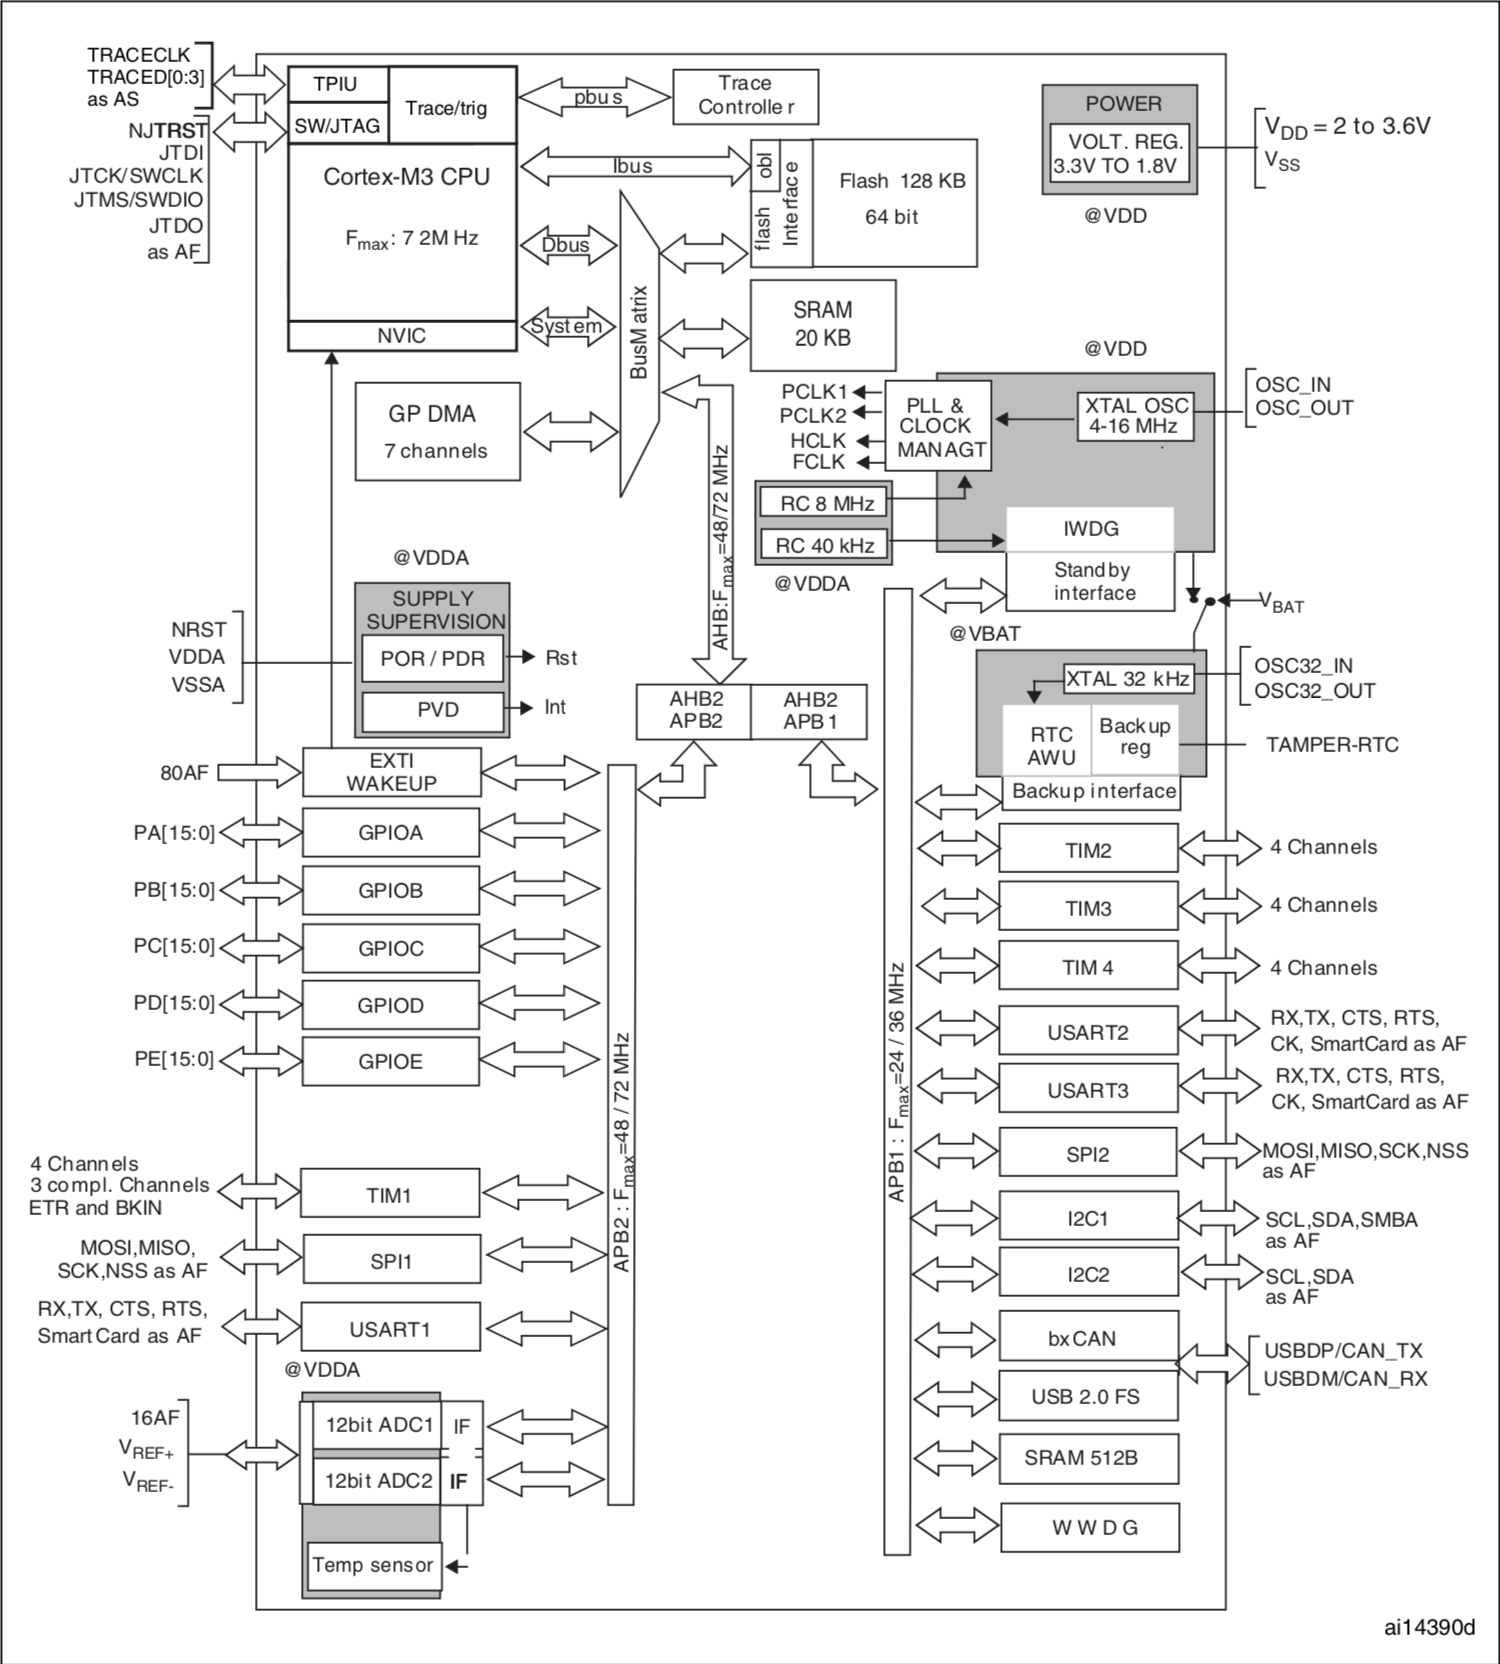
\includegraphics[width=\textwidth]{images/content/clockDiag.png}
			\captionof{figure}{STM32时钟线}
			\label{fig:clockDiag}
		\end{figure}
	
	\subsection{GPIO的输出操作}
		配置为推挽或开漏输出模式的引脚,可以控制其输出高电平或低电平,与之相关的库函数有下面几个:
		\par 
		\begin{lstlisting}[language=bash, style=customStyleC]
/*控制整个GPIO端口的输出值*/
void GPIO_Write(GPIO_TypeDef * GPIOx, uint16_t PortVal);

/*控制某个引脚的输出值*/
void GPIO_WriteBit(GPIO_TypeDef * GPIOx, uint16_t GPIO_Pin, 
	BitAction BitVal );

/*拉高(置位,set)某些引脚*/
void GPIO_SetBits(GPIO_TypeDef* GPIOx, uint16_t GPIO_Pin);

/*拉低(复位,reset)某些引脚*/
void GPIO_ResetBits(GPIO_TypeDef* GPIOx, uint16_t GPIO_Pin);
		\end{lstlisting}
		\par 
		其中,第1个函数改变整个端口16个引脚的输出值,因此它的第二个参数是一个16位的无符号整数,从第15位到第0位分别对应某一端口第15号引脚到第0号引脚,这种操作一般用于手工进行并行数据传输。第2个函数改变某个引脚的输出值,其第三个参数决定是拉高(对应Bit\_SET)还是拉低(对应Bit\_RESET),不过这个函数只能操作某一个引脚。后两个函数分别拉高、拉低某些引脚,第二个参数为用按位或运算符连接的若干引脚,当然,控制单个引脚也是可以的。
		\par 
		下面,我们看看如何用这些函数来控制GPIO完成点亮LED灯的操作。以下两个函数位于GPIO.c文件中。
		\par 
		\begin{lstlisting}[language=bash, style=customStyleC, caption=LED控制操作]
void LED1Operation(u8 on) {
	if(on) {
		GPIO_ResetBits(GPIOA, GPIO_Pin_0);
	} else {
		GPIO_SetBits(GPIOA, GPIO_Pin_0);
	}
}

void LED2Operation(u8 on) {
	GPIO_WriteBit(GPIOA, GPIO_Pin_1, on ? Bit_RESET : Bit_SET);
}
		\end{lstlisting}
		\par 
		这里,控制LED1的函数用了直接拉高、拉低引脚的库函数,而控制LED2的函数则使用了写入某一引脚的库函数。需要注意,也许有的读者知道Bit\_SET和Bit\_RESET的值(分别为1和0)之后会想到把上述代码第10行的三元表达式替换为1 - on甚至是1 \^{} on(位异或运算),但实际上,我们使用了8位整型来表达布尔类型,因此任何非零值都应理解为真,如果做出这样的替换,就相当于限制了参只能传入0或1。有时为了较高的性能我们确实会这么做,但一般来说,这是不建议的。
		
	\subsection{GPIO的读入操作}
		配置为浮空输入、上拉输入或者下拉输入模式的引脚,可以读取输入的电平高低,与之相关的库函数有下面几个:
		\par 
		\begin{lstlisting}[language=bash, style=customStyleC]
/*读取某个引脚上的输入电平*/
uint8_t GPIO_ReadInputDataBit(GPIO_TypeDef* GPIOx, uint16_t GPIO_Pin);

/*读取整个GPIO端口的输入值*/
uint16_t GPIO_ReadInputData(GPIO_TypeDef* GPIOx);
		\end{lstlisting}
		\par 
		第一个函数读取某个引脚上的输入电平,高电平返回Bit\_SET,低电平返回Bit\_RESET。第二个函数读取整个GPIO端口的输入数据,返回一个16位无符号数,从第15位到第0位分别对应某一端口第15号引脚到第0号引脚上的输入电平。
		\par 
		下面我们看看如何用这些函数检测按键是否被按下了。
		\par 
		\begin{lstlisting}[language=bash, style=customStyleC, caption=按键检测]
u8 Button1Pressing() {
	return GPIO_ReadInputDataBit(GPIOA, GPIO_Pin_2) == Bit_SET;
}

u8 Button2Pressing() {
	return GPIO_ReadInputDataBit(GPIOA, GPIO_Pin_3) == Bit_RESET;
}
		\end{lstlisting}
		\par 
		函数的功能简明易懂,但这样,能够完美地实现检测按键的功能吗?
		
	\subsection{按键的抖动}
		由于按键是一种机械结构触发的电子开关,当人手按下按键时,相应信号并不会立即跳变,而是会迅速发生几次跳变,而后稳定下来,当松开按键时,也会发生同样的情况,这就是按键的抖动,形象的描述见图\ref{fig:keyShake}\footnote{http://mooc.chaoxing.com/nodedetailcontroller/visitnodedetail?knowledgeId=630317}。这种抖动可能使我们重复检测到按键按下的事件,甚至在松开按键的过程中也会这样,因此,必须想办法消除这种影响。
		\begin{figure}[h]
			\begin{center}
				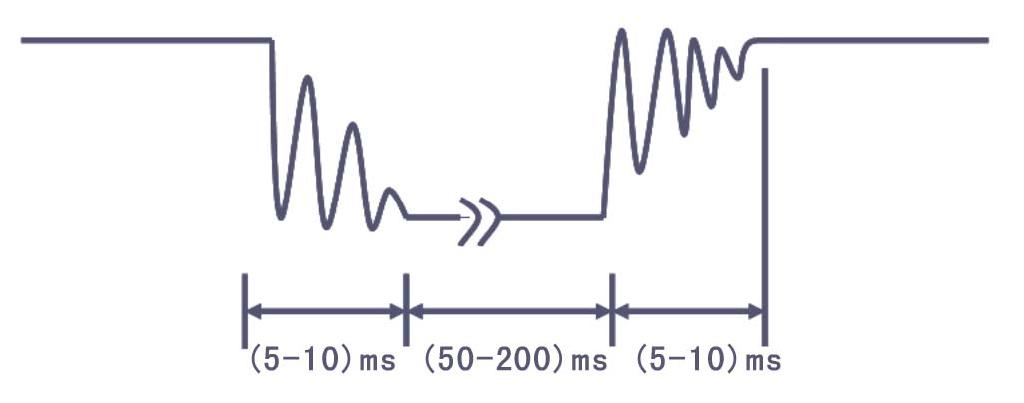
\includegraphics[width=110mm]{images/content/keyShake.jpg}
				\captionof{figure}{按键抖动}
				\label{fig:keyShake}
			\end{center}
		\end{figure}
		\par 
		我们可以使用一些数字电路来消除这种抖动带来的影响,但这样过于复杂。我们也可以用软件的方式来实现同样的目的,即检测到电平变换后,延时一定时间(例如50ms),再检测一遍,如果仍为按下状态,则认为按键已经按下,否则认为没有按下。但在此之前,让我们想想如何进行延时的操作,要知道,单片机里可没有<time.h>之类的操作。
	
	\subsection{循环的延时作用}
	想要延时,最简单的方法是让程序执行相当多次什么也不干的循环。经过几次调参,一个简易的延时函数如下所示:
		\par 
		\begin{lstlisting}[language=bash, style=customStyleC, caption=简易延时函数]
void delay(volatile uint32_t ms) {
	volatile uint32_t i, j;
	for(i = 0; i < 6000; ++i) {
		for(j = 0; j < ms; ++j);
	}
}
		\end{lstlisting}
		\par 
		一个优秀的编译器在吸了氧气(指开启-O2优化)之后可能会把空循环甚至幂等的循环(即循环一次与循环多次等价)直接优化掉,因此我们一定要声明变量为volatile的。有了这个延时函数,我们就可以解决按键抖动问题了。
	
	\subsection{消抖后的按键检测}
		\par 
		\begin{lstlisting}[language=bash, style=customStyleC, caption=消抖后的按键检测函数]
u8 Button1Pressing() {
	if(GPIO_ReadInputDataBit(GPIOA, GPIO_Pin_2) == Bit_SET) {
		delay(50);
		return GPIO_ReadInputDataBit(GPIOA, GPIO_Pin_2) == Bit_SET;
	} else return 0;
}

u8 Button2Pressing() {
	if(GPIO_ReadInputDataBit(GPIOA, GPIO_Pin_3) == Bit_RESET) {
		delay(50);
		return GPIO_ReadInputDataBit(GPIOA, GPIO_Pin_3) == Bit_RESET;
	} else return 0;
}
		\end{lstlisting}
		\par 
		上面这两个函数的实现思路与之前的分析一致,使用延时的方法来消除抖动的影响。
		\par 
		至此,我们已经实现了LED灯的控制以及按键检测的功能,下面,我们就可以用这些函数来实现各种各样的效果了。
	\subsection{功能的实现}
		想要实现我们希望的功能,需要编辑main.c文件,这是程序的入口main()函数所在的位置。我们需要将程序的逻辑写在main()函数内部。不过,在编辑main()函数之前,我们需要在文件开头包含刚刚编写的GPIO.h头文件。
		\par
		首先,让我们看看实现一个LED灯闪烁功能的程序:
		\par
		\begin{lstlisting}[language=bash, style=customStyleC, caption=LED灯闪烁]
int main(void) {
	PinsInit();
	LED2Operation(0);
	while(1) {
		LED1Operation(1); delay(500);
		LED1Operation(0); delay(500);
	}
}
		\end{lstlisting}
		\newpage
		\par 
		程序首先调用初始化函数对用到的引脚进行初始化,然后将LED2熄灭,此后进入一个无限循环,在这个循环中,以大约1秒为周期交替点亮、熄灭LED1。如果编译并下载这个程序,正确地连接电路,我们就可以看到LED闪烁的效果了。这里我们使用的delay()函数与之前实现的一样。

















